\chapter{Cloudooo}
\label{cap4}

O Cloudooo é um serviço Web desenvolvido neste trabalho que utiliza o protocolo XML-RPC para troca de mensagens. Esta aplicação, desenvolvida em Python, provê a extração e inserção de metadados em um documento e a conversão do mesmo para qualquer formato suportado pelo OpenOffice.org. É um projeto de código aberto que se encontra sob a licença LGPL.

Cada parte da aplicação pode ser utilizada separadamente ou em outra aplicação. Estas partes são dividas em oito interfaces:
\begin{itemize}
\item \textit{IManager} é a declaração de todos os métodos que o usuário pode utilizar;
\item \textit{IDocument} representa cada documento que o servidor recebe;
\item \textit{IHandler} representa objetos que irão fazer todo trabalho que é pedido pela requisição de um cliente; 
\item \textit{ILockable} define métodos para controle de uma determinada região que não pode ser acessada por mais de um cliente. Isto é utilizado em casos de serviços com grande demanda que necessitam ter controle do uso dos recursos disponibilizados; 
\item \textit{IMonitor} define métodos para controle e manuseio dos processos;
\item \textit{IMimemapper} fornece métodos para manusear todos filtros existentes no OpenOffice.org;
\item \textit{IApplication} define métodos para controle de aplicativos externos ao serviço Web;
\item \textit{IFilter} representa cada filtro do \textit{software} OpenOffice.org;
\end{itemize}

Cada uma dessas interfaces e suas implementações são explicadas nas subseções seguintes.

\section{\textit{IApplication}}
\label{iapp}
Para um melhor controle dos processos externos ao Cloudooo é necessário que métodos possam não só iniciar e parar o processo, mas também saber a qualquer momento se o mesmo está rodando no sistema operacional, o seu identificador e qual porta do sistema ele está usando. No caso do Cloudooo também era necessário que a configuração do processo seja dinâmica. Desta forma, além dos métodos básicos de controle de um processo, foi inserido o método \textit{loadSettings} para que seja possível configurar o processo da melhor maneira.

\subsection{OpenOffice e Xvfb}
\label{obj:openoffice}

Com a necessidade de um aplicativo \textit{desktop} em um ambiente de produção, sendo na maioria dos casos servidores que não possuem interface gráfica instalada, é necessário que nesses ambientes o aplicativo fique sempre aberto e funcional. Para que isso seja possível, estes ambientes  de produção exigem uma interface gráfica para que o OpenOffice.org fique aberto e possibilite que a partir somente do identificador da interface, seja possível abrir qualquer aplicativo nesta interface gráfica em memória.

Portanto, a classe Xvfb é responsável por controlar a interface gráfica em memória e a classe OpenOffice utiliza este para abrir o aplicativo. As Figuras \ref{exemplo:xvfb} e \ref{exemplo:openoffice} apresentam exemplos de uso de ambos os objetos.

\begin{figure}[ht]
\centering
\begin{center}
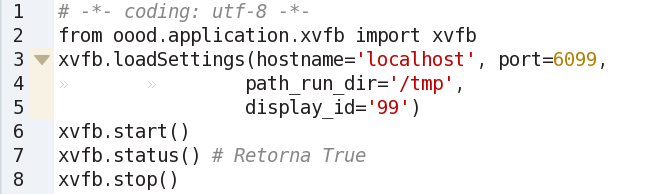
\includegraphics[scale=0.65,bb=0 0 550 156]{xvfb_exemplo.png}
\end{center}
\caption{Utilização da API \textit{IApplication} para controlar o processo Xvfb.}
\label{exemplo:xvfb}
\end{figure}

\begin{figure}[ht]
\centering
\begin{center}
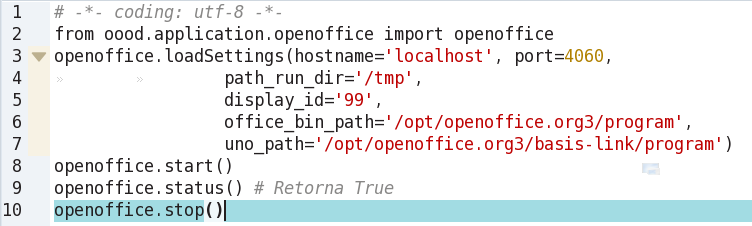
\includegraphics[scale=0.65,bb=0 0 550 156]{openoffice_exemplo.png}
\end{center}
\caption{Utilização da API \textit{IApplication} para controlar o processo OpenOffice.org.}
\label{exemplo:openoffice}
\end{figure}

Nota-se que, na Figura \ref{exemplo:openoffice} existem dois parâmetros de configuração declarados na linha 6 e 7, que não constam na Figura \ref{exemplo:xvfb}. O identificador da interface gráfica, com nome de \textit{display\_id}, em ambos os exemplos são iguais. Essas diferenças de controle entre o processo Xvfb e OpenOffice.org, são justificadas pelo fato de que o OpenOffice precisa do identificador da interface gráfica para iniciar o aplicativo OpenOffice.org e além disso, o caminho do binário do mesmo e da bibliteca UNO.

\section{\textit{IManager}}
\label{obj:manager}

A interface \textit{IManager} é o contrato entre cliente e servidor. Com o objetivo de um contrato mais genérico, foram declarados métodos que futuramente pudessem trabalhar com outros tipos de dados além de documentos. Então, caso a aplicação Web seja estendida para trabalhar, por exemplo, com conversão de vídeos e imagens, o cliente não é afetado.

\subsection{\textit{Manager}}

O classe \textit{Manager} é responsável por criar tarefas enviadas pelo cliente. A Figura \ref{exemplo:manager} apresenta um exemplo da criação de uma tarefa simulando um cliente.

\begin{figure}[ht]
\centering
\begin{center}
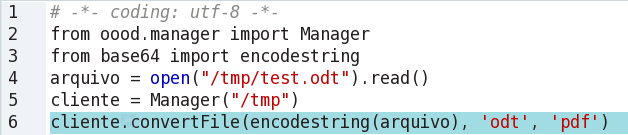
\includegraphics[scale=0.75,bb=0 20 500 85]{manager_exemplo.png}
\end{center}
\caption{Exemplo de utilização do objeto \textit{Manager}.}
\label{exemplo:manager}
\end{figure}

Note que nesta mesma figura, uma biblioteca de codificação é utilizada, chamada \textit{base64}. Esta biblioteca tem como objetivo codificar os dados para transferência pela internet, pois a rede de computadores não suporta o tráfego de documentos em seu estado original.

Como os documentos recebidos pelo objeto \textit{Manager} estão codificados em \textit{base64}, antes de serem salvos no sistema de arquivo, são descodificados para retornar ao estado original. Além disso, os documentos retornados para o usuário também são codificados para serem enviados via rede.

\section{\textit{IDocument}}
No serviço de aplicação OOOD, a prioridade é uma resposta eficiente e consistente ao cliente. Para que isso seja possível é necessário que haja integridade total nos dados enviados para o servidor. Com estes requisitos, a \textit{IDocument} propõe um contrato em que é possível saber o contéudo do documento, atualizá-lo e em casos de problemas em tempo real, recuperar o documento original.

\subsection{\textit{FileSystemDocument}}
\label{fsd}
A classe \textit{FileSystemDocument} utiliza a própria estrutura de pastas do sistema operacional como forma de armazenar os dados. Os arquivos são postos em pastas temporárias que são deletadas quando o objeto não é mais utilizado. Desta forma, cada pasta representa uma requisição do cliente. A Figura \ref{exemplo:fss} demonstra como utilizar este objeto para manipular documentos no sistema de arquivo.

\begin{figure}[!ht]
\centering
\begin{center}
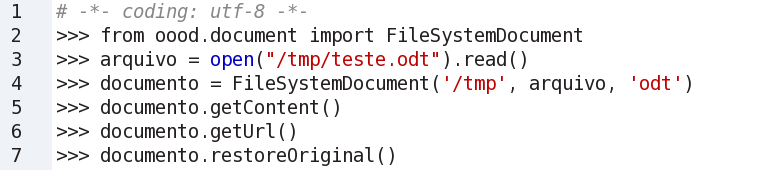
\includegraphics[scale=0.677,bb=0 0 490 95]{fss_exemplo.png}
\end{center}
\caption{Exemplo de uso do \textit{FileSystemDocument}.}
\label{exemplo:fss}
\end{figure}

\section{\textit{IMonitor}}

Com a dificuldade de controle dos processos e os constantes erros que afetavam toda a aplicação, a interface \textit{IMonitor} definiu um contrato que, com atributos mínimos, torna possível monitorar o processo e obter informações à partir disso. Com isso, é possível criar monitores que fiscalizam uma parte da aplicação e caso haja algum resultado não esperado, o pode ser corrigido.

A subseções seguintes apresentam monitores implementados para controlar cada tipo de problema. Portanto, em cada subseção será mostrado o problema e a solução para o mesmo.

\subsection{\textit{MemoryMonitor}}

Com o uso excessivo da conexão entre o OpenOffice.org e o UNO, em muitos casos, a memória utilizada para troca de mensagens não era liberada. Esta falha é a causa de um fenômeno, chamado de vazamento de memória ou \textit{memory leak}, que ocorre em sistemas computacionais quando uma porção de memória alocada para uma determinada operação, não é liberada quando não é mais necessária \cite{1211498}. A consequência disto é o uso de toda memória do computador. 

Para o controle deste problema, a classe \textit{MemoryMonitor} é responsável por fiscalizar a memória utilizada pelo OpenOffice.org e caso esta memória aumente de forma descontrolada o processo é parado imediatamente e reiniciado. Em suma, esta solução foi adicionada pois o sistema operacional não é programado para detectar essas falhas, sendo este erro acusado somente quando toda memória do computador é utilizada.

\subsection{\textit{TimeoutMonitor}}

Com o uso excessivo do OpenOffice.org foi detectado que existem momentos que o mesmo não consegue abrir um documento, pois está travado. Então, a classe \textit{TimeoutMonitor} tem como objetivo limitar o tempo de uso do OpenOffice.org para não permitir que a requisição do cliente fique esperando a resposta por tempo indeterminado. Caso o uso do OpenOffice.org extrapole o tempo máximo, o OpenOffice.org é reiniciado e a requisição é enviada novamente.

\subsection{\textit{RequestMonitor}}

Com o comprometimento da estabilidade do aplicativo à partir de muitas requisições respondidas pelo OpenOffice.org, foi implementado a classe \textit{RequestMonitor}, que reinicia o OpenOffice.org quando o número de requisições respondidas chega ao limite.

\section{\textit{ILockable}}

A exclusão mútua é uma técnica de programação que está inserida em um paradigma de programação chamado de programação concorrente. Esta técnica tem como objetivo impedir que processos ou \textit{threads} tenham acesso a um recurso compartilhado, garantindo a consistência e integridade dos dados \cite{355074}. Este trecho ou recurso compartilhado é chamado de região crítica. Portanto, a interface \textit{ILockable} propõe métodos para controlar a região crítica.

\subsection{OpenOffice}

Além de implementar a interface \textit{IApplication}, descrita na sessão \ref{iapp}, a classe OpenOffice necessita controlar o uso do aplicativo OpenOffice.org, pois este não pode atender mais de uma requisição ao mesmo tempo. Sendo assim, para que haja controle no uso do aplicativo, a classe OpenOffice implementa esta interface, como demonstra a Figura \ref{fig:oo_lockable} o uso de métodos da \textit{ILockable} para controlar o objeto.

\begin{figure}[!ht]
\centering
\begin{center}
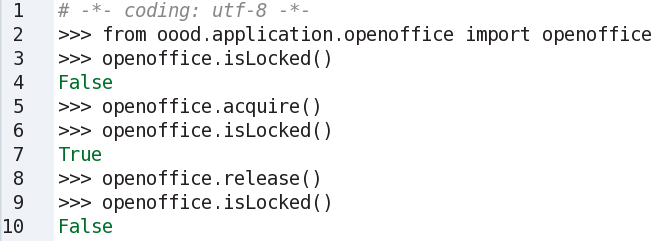
\includegraphics[scale=0.610,bb=0 0 500 146]{open_lockable.png}
\end{center}
\caption{Exemplo de uso da interface \textit{ILockable} no objeto OpenOffice.}
\label{fig:oo_lockable}
\end{figure}

\section{\textit{IHandler}}

Com a necessidade de uma arquitetura flexível, além de fazer com que cada objeto tenha somente uma responsabilidade, foi criada uma interface que é o contrato para objetos responsáveis pela conversão de dados, como por exemplo documentos, vídeos e imagens.

\subsection{\textit{OOHandler}}

A classe \textit{OOHandler} é implementada para comunicar-se com o OpenOffice.org. Quando o serviço OOOD recebe uma requisição, ele automaticamente delega estes dados para o \textit{OOHandler} e requista ao mesmo objeto algum procedimento, por exemplo extrair metadados. Além disso, para armazenar e manusear os dados enviados pelo cliente, o \textit{OOHandler} possui um objeto \textit{FileSystemDocument}, pois caso ocorra falhas, estes dados podem ser restaurados. A Figura \ref{fig:ex_oohandler} demonstra um exemplo de utilização do \textit{OOHandler} e o documento com um objeto \textit{FileSystemDocument}.

\begin{figure}[!ht]
\centering
\begin{center}
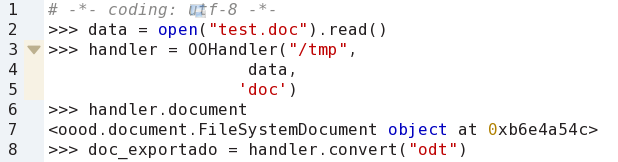
\includegraphics[scale=0.750,bb=0 10 500 106]{ex_oohandler.png}
\end{center}
\caption{Exemplo de utilização do \textit{OOHandler}.}
\label{fig:ex_oohandler}
\end{figure}

\section{\textit{IMimemapper}}

Antes do documento ser aberto pelo OpenOffice.org, existe um pré-processamento para saber o formato do arquivo. Este pré-processamento é necessário, pois para cada extensão existe um filtro específico. 

Em um sistema \textit{desktop} comum, os nomes dos arquivos incluem uma extensão que indica o formato do arquivo, por exemplo ``document.doc''. Antes de abrí-lo na suíte de aplicativos do OpenOffice.org, a suíte detecta a extensão pelo nome do arquivo e através disto abre o arquivo com o filtro referente ao formato. Em casos que o nome do arquivo não define a extensão, o OpenOffice.org tenta descobrir o formato, caso contrário ocorre uma falha dizendo que o arquivo não pode ser aberto pelo aplicativo.

Portanto, com o objetivo de criar um ambiente parecido com um sistema \textit{desktop}, o \textit{IMimemapper} provê métodos para obter todas informações necessárias para manipular um documento antes mesmo de carregá-lo no OpenOffice.org.

\subsection{Filtros do OpenOffice.org}
O aplicativo OpenOffice.org utiliza a linguagem XML para armazenar filtros, extensões e tipos de arquivos. Numa instalação normal, o OpenOffice.org armazena todos esses dados dentro da pasta \textit{TypeDetection} que localiza-se dentro da estrutura de pastas da instalação. Por exemplo, ao utilizar o pacote oficial de instalação, o caminho completo desta pasta seria ``/opt/openoffice.org/basis3.1/share/registry/modules/org/openoffice/TypeDetection''.

Dentro da pasta \textit{TypeDetection} existem duas pastas, que são \textit{Filter} e \textit{Types}. A pasta \textit{Filter} armazena os filtros e o serviço utilizado para exportar um documento utilizando este filtro e \textit{Types} armazena as propriedades de um filtro. As Figuras \ref{fig:type1} e \ref{fig:filter}, demonstram, respectivamente, um exemplo de filtro e tipo declarado no OpenOffice.org. Estes exemplos serão utilizados para explicação dos dados relevantes usados para o Cloudooo.

\begin{figure}[!ht]
\centering
\begin{center}
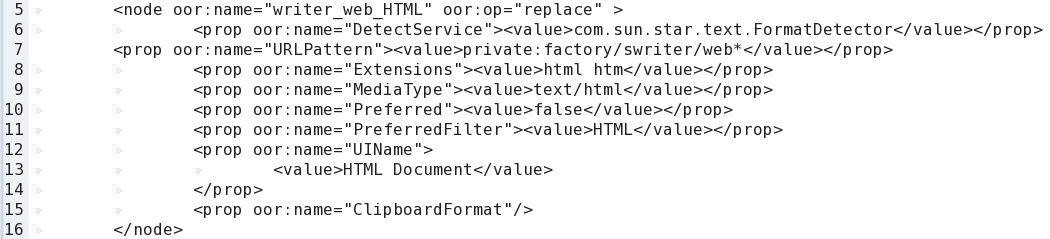
\includegraphics[scale=0.610,bb=0 0 750 166]{type1.jpg}
\end{center}
\caption{Propriedades de um filtro.}
\label{fig:type1}
\end{figure}

\begin{figure}[!ht]
\centering
\begin{center}
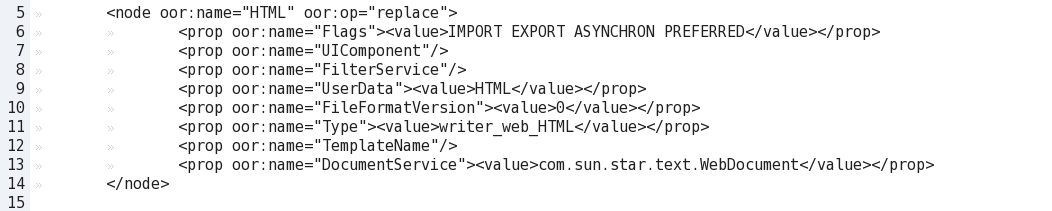
\includegraphics[scale=0.610,bb=0 0 750 146]{filter.jpg}
\end{center}
\caption{Exemplo de um filtro do OpenOffice.org.}
\label{fig:filter}
\end{figure}

Os dados apresentados nas figuras \ref{fig:type} e \ref{fig:filter}, são dados que analisando-os é possível saber qual extensão terá o arquivo caso seja exportado utilizando este filtro. 
\paragraph{}

A ligação entre filtro e tipo é feita pela propriedade \textit{Type} declarado na linha 11 da Figura \ref{fig:filter} e o nome do nó, declarado na linha 5 da Figura \ref{fig:type}. Então, com esta associção, utilizando o filtro HTML o documento terá formato ``htm'' ou ``html'', pois estas extensões estão declarados na propriedade \textit{Extensions}, situado na linha 8 da Figura \ref{fig:type}.
\subsection{\textit{Mimemapper}}
\label{obj:mimemapper}

O UNO possui metódos que possibilitam extrair diversos tipo de informação do OpenOffice.org. A partir disto, a classe \textit{Mimemapper} é responsável por utilizar estes metódos para obter todos os dados necessários para importar e/ou exportar documentos. A Figura \ref{fig:load} apresenta como os filtros são carregados para o \textit{Mimemapper}.

Com os filtros carregados, estes são armazenados em objetos do tipo \textit{Filter}, descrito na sessão \ref{obj:filter}, com o objetivo de tornar fácil o acesso as informações e oferecer uma maior flexibilidade na busca. Por exemplo, na linha 5 da Figura \ref{fig:load}, a partir de informações sobre um determinado formato de arquivo, é possível saber qual nome do filtro é utilizado para importar ou exportar um documento no mesmo formato.

\begin{figure}[!ht]
\centering
\begin{center}
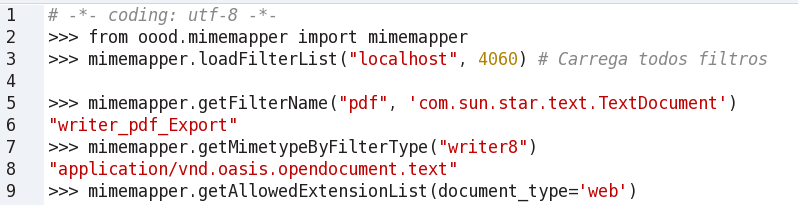
\includegraphics[scale=0.74,bb=0 0 580 140]{mime_load.png}
\end{center}
\caption{Importando todos filtros do OpenOffice.org para o \textit{Mimemapper}.}
\label{fig:load}
\end{figure}


\section{\textit{IFilter}}
\label{interface:filter}

Quando o \textit{Mimemapper}, descrito na sessão \ref{obj:mimemapper}, extrai os filtros do OpenOffice.org, cada um contêm informações que serão utilizadas durante todo o uso da aplicação, mas esses dados precisam ser armanazenados de forma segura e de fácil manuseio. Para isso criou-se um contrato para que cada filtro seja um objeto e tenha métodos que possam extrair suas informações da melhor forma possível.

\subsection{\textit{Filter}}
\label{obj:filter}
O \textit{Filter} é a classe implementada mais simples de toda aplicação. Seu propósito é armazenar todas informações que um filtro do OpenOffice.org possui. A Figura \ref{fig:type} é um exemplo de como criar um filtro e extrair informações do mesmo através do métodos declarados na interface \textit{IFilter}.

\begin{figure}[!ht]
\centering
\begin{center}
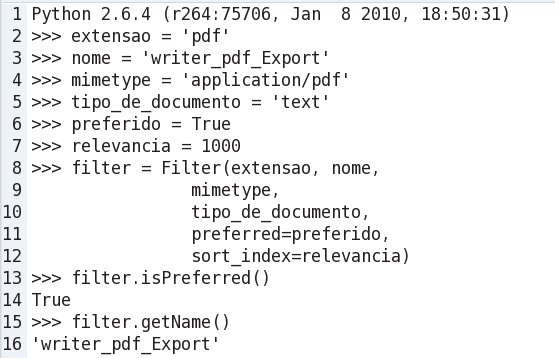
\includegraphics[scale=0.710,bb=0 0 500 250]{exemplo_filter.png}
\end{center}
\caption{Exemplo de criação de um objeto \textit{Filter}.}
\label{fig:type}
\end{figure}